% main.tex
\documentclass[14pt]{article}
\usepackage{pepadun}
\usepackage{glossaries}
\usepackage{amsmath}
\newcommand{\norm}[1]{\left\lVert#1\right\rVert}
\makeglossaries

\makeglossaries
\newglossaryentry{Laue's theory}
{
    name=Laue's theory,
    description={Laue's Law is a fundamental principle in X-ray diffraction used to describe the scattering of X-rays by a crystal lattice. It states the conditions that must be met for constructive interference to occur when a beam of X-rays interacts with the regularly spaced atoms in a crystal.In terms of the reciprocal lattice, the condition for diffraction is that the difference between the incident wave vector ($\mathbf{k}$) and the scattered wave vector ($\mathbf{k'}$) must equal a reciprocal lattice vector ($\mathbf{G}$).}
}

\newglossaryentry{Laue's equation}{
    name= Laue's equation,
    description= {The three Laue Equations are the scalar expressions that must be simultaneously satisfied for constructive interference to occur when X-rays are diffracted by the periodic structure of a crystal lattice.They represent the condition that the path difference between waves scattered from adjacent atoms along each of the three crystal axes ($\mathbf{a}$, $\mathbf{b}$, $\mathbf{c}$) must be an integral multiple of the X-ray wavelength ($\lambda$).The equations are:$$a(\cos\alpha - \cos\alpha_0) = h\lambda \\
b(\cos\beta - \cos\beta_0) = k\lambda \\
c(\cos\gamma - \cos\gamma_0) = l\lambda$$Where:$a, b, c$ are the primitive translation lengths (lattice constants) along the crystal axes.$\cos\alpha_0$, $\cos\beta_0$, $\cos\gamma_0$ are the direction cosines of the incident X-ray beam with respect to the crystal axes.$\cos\alpha$, $\cos\beta$, $\cos\gamma$ are the direction cosines of the diffracted X-ray beam with respect to the crystal axes.$h, k, l$ are integers (now known to be equivalent to the Miller indices of the diffracting plane).$\lambda$ is the X-ray wavelength.These three scalar equations are mathematically equivalent to the single vector form of Laue's Law, which states that the change in the wave vector must equal a reciprocal lattice vector $\mathbf{G}$:$$\mathbf{k'} - \mathbf{k} = \mathbf{G}$$}
}

\newglossaryentry{Miller Indices}{
    name= Miller indices,
    description={Miller Indices are a system of notation in crystallography that uses three integers to uniquely identify the orientation of a family of parallel planes within a crystal lattice.They are derived from the reciprocals of the fractional intercepts that a plane makes with the three crystallographic axes ($\mathbf{a}$, $\mathbf{b}$, $\mathbf{c}$).A set of Miller indices $(hkl)$ for a plane is fundamentally equivalent to identifying a vector in the reciprocal lattice, $\mathbf{G}_{hkl}$, which is perpendicular to that plane.The plane's equation, in terms of its fractional intercepts $(a/h, b/k, c/l)$ along the crystal axes, satisfies:$$\frac{x}{a/h} + \frac{y}{b/k} + \frac{z}{c/l} = n \quad \text{or, more generally, } \quad h\frac{x}{a} + k\frac{y}{b} + l\frac{z}{c} = n$$where:$(hkl)$ are the Miller Indices (always integers, often reduced to the smallest set).$n$ is an integer (the $n$-th plane from the origin).A bar over an index (e.g., $\bar{h}$) denotes a negative intercept.Round brackets $\mathbf{(hkl)}$ denote a single plane or a family of parallel planes.Curly brackets $\mathbf{\{hkl\}}$ denote a family of equivalent planes (by crystal symmetry).They are essential for interpreting X-ray diffraction patterns, as the diffraction condition (Laue's Law) directly relates the change in the wave vector to a reciprocal lattice vector $\mathbf{G}_{hkl}$, which is indexed by $h, k, l$.}
}


% \usepackage[backend=biber, style=ieee]{biblatex}
% \addbibresource{pepadun.bib}  % Gunakan file bib yang disediakan

% Metadata dokumen
\title{Bragg's Law in the Context of Protein Structure Determination}
\author{%
    \begin{tabular}{c}
        Loredana-Maria Iacob, \\
        Chemistry and Biotechnology, School of Science, \\
        Constructor University \\ 
        \\
        e-mail:  liacob@constructor.university, \\
    \end{tabular}
}
\date{April 30th, 2025} % Hapus tanggal otomatis

\begin{document}

\maketitle

\begin{abstract}
Scientists lacked a clear understanding of how waves interact with atoms and crystals. Analyzing diffraction peaks determines the spacing between atomic planes and, consequently, the crystal's structure. The father and son team of William Henry Bragg and William Lawrence Bragg were the first to correctly analyze the diffraction peaks pattern. \\
This paper introduces Bragg's law in the context of X-ray Crystallography. It outlines the protein structure determination by crystallization, Fourier analysis of diffraction intensities, and finally solving the electron density map. Even in a field where mathematics is assumed to be absent, this paper illustrates the power of mathematical construction and its unforeseen applicability to complex systems and real-world phenomena.
\end{abstract}

\section{Introduction to the fundamental problem of determining atomic-scale crystal structures}

Scientists lacked a clear understanding of how waves interact with the atomic planes in a crystal. Analysing diffraction peaks determines the spacing between atomic planes and, consequently, the crystal's structure. Numerous experiments and theories have been tested before a concise explanation of the interaction between X-Ray and atoms or plans of atoms have been found.
The father and son team of William Henry Bragg and William Lawrence Bragg were the first to attempt determining crystal structures using X-rays. They did this in 1913, utilizing X-ray diffraction to reveal how atoms are arranged within crystals. W. L. Bragg, inspired by Max von Laue and his experiments with X-Ray, proposed a corrected version of Laue's theory that he later used to prove Bragg's Law and form the basis of what we call today X-ray crystallography.

This discovery led to many of the most important scientific achievements of the last century, and these continue to the present day. This paper was the beginning of the field of X-ray crystallography, a subject that has enabled us to establish the complete structures of crystals, starting from the very simple to the most complex materials, such as proteins, viruses and the molecule that forms the very essence of life, namely DNA.
Around 20 or so Nobel Prizes have been awarded for research that has used the ideas described by Bragg. Modern genetics, medicine and the study of materials owe an incalculable debt to WLB, who at the astonishingly young age of 22, made a discovery that has changed our understanding of the world around us. Both father and son shared the 1915 Nobel Prize for their work, with WLB remaining to the present day the youngest Nobel Prize winner ever.

\section{Bragg's experiments and observations}

His paper starts with an overview of The Laue experiment, published in \cite{Friedrich} “Interference Phenomena with Räntgen Rays” published by Herren Friedrich et. al., in which a beam of X-ray was passed through a crystal of simple structure and rectilinear pencils (narrow beams or rays of X-ray with a focused and controlled nature) were observed to spread in all directions forming a geometric pattern. The spots (where the maxima points hit the photographic plate) remain symmetric to the axes of a cubical zinc blade, when the ray is perpendicular to the third axis as shown in Figure \ref{fig:Plate II}. After further analysis of the plate and geometric relationships between the spots and crystal structures, it was noticed that the spots are points of intersection between ellipsis. Bragg explains the formation, shape and position of these ellipsis with a few geometric formulas.\\

\begin{figure}[h]
    \centering
    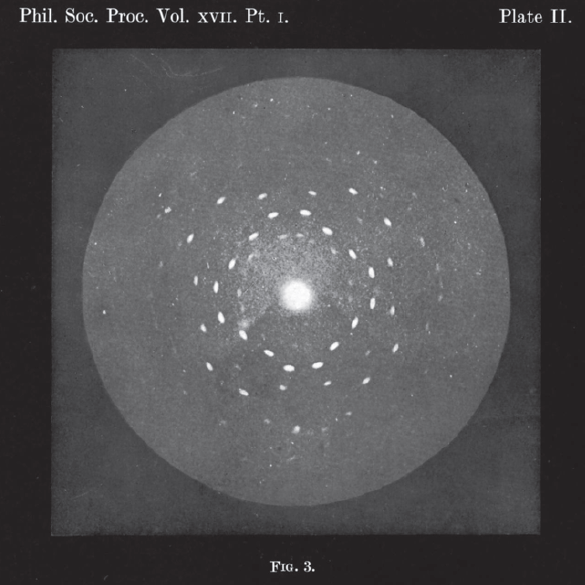
\includegraphics[width=0.5\linewidth]{Captură de ecran 2025-04-21 151112.png}
    \caption{Plate II}
    \label{fig:Plate II}
\end{figure}

\gls{Laue's theory} is that secondary X-rays are emitted by molecules, and these interfere to form a patter according to the system :
$$a \alpha =h_1 \lambda$$
$$b \beta = h_2 \lambda$$
$$c(1- \gamma) = h_3 \lambda$$

Where $h_1, h_2, h_3$ are integers, a is the side of the cube, $\lambda$ the wavelength of the secondary waves and $\alpha$, $\beta$, $\gamma$, are the directional cosine of the new maxima. Note that the waves are parallel to the z axis so the surface of the beam parallel to the xy plane. Also, even though the system is technically correct, it was made with the wrong assumption that the atoms emit secondary waves, but these waves are in fact the ones reflected by the planes of the crystal, as it was later proved. 

This system suggests that all secondary waves are in phase in the direction of whose cosines are $\alpha, \beta, \gamma$. The experimental set up allowed to calculate these values and prove the existence of such integers.
However, not all $h_1, h_2, h_3$ are represented. Laue assumed that only certain $\lambda$ are represented because $\frac{\lambda}{a}$ also has to be an integer, but his assumption is wrong. Firstly, only certain $\lambda$ are present in the incident beam and, secondly, there are integers corresponding to certain $\frac{\lambda}{a}$ that do not appear in the pattern.\\
WLB makes the correct assumption that a continuous range of $\lambda$ are present and then proved, with the law he formulates, why such a beam does not form a uniform darkness. He suggests that X-rays are reflected by “centres of disturbance” (i.e. plans of atoms), the same way as light, and the reflected pulse interferes with the incoming ones to build a front.

Considering plans of atoms in the crystal, the reflected beams from each plane can be seen to interfere after being reflected to a $\theta$ angle in planes found at distance d of each 0ther. The formed wavelengths are $\lambda, \frac{\lambda}{2}, \frac{\lambda}{3}, \frac{\lambda}{4}$ etc, where
$$\lambda=2d \cos{\theta}$$
The intensity of a spot depends on the “average breadth” of the beam, such us if $2d \cos{\theta}$ is too small, pulses will neutralize each other, and if it is too big, they will be too far from each other. Thus, the reflections occur for specific combinations of $\lambda, d, \theta$ and this is why the plate does not show a uniform darkness.

\begin{figure}[h]
    \centering
    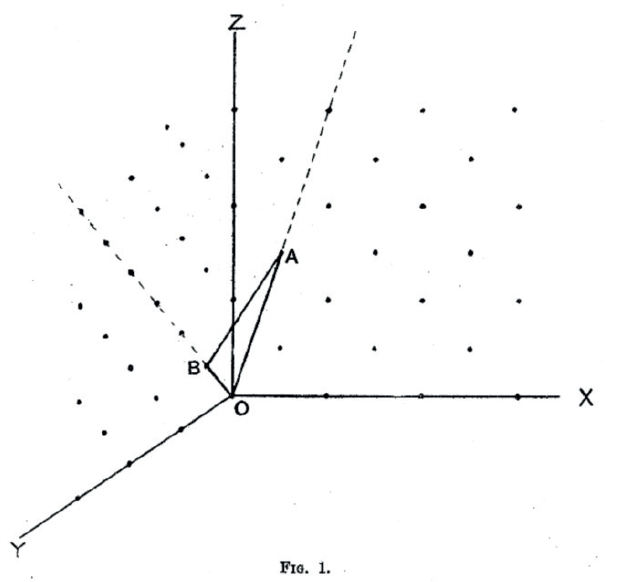
\includegraphics[width=0.5\linewidth]{Captură de ecran 2025-04-21 154041.png}
    \caption{Crystal planes O(0,0,0), B(0,a,a), A(a,0,3a) showing the link between the angle of incidence and the directional cosines of the plane}
    \label{fig:planes}
\end{figure}

Designing his experiment, WLB uses the Pope and Barlow theory to assume arrangements of atoms in a zinc blende and assumes that zinc and sulfur emit secondary waves of the same power to explain why some $\lambda$ miss in Laue’s model. Taking the cubic packed model, with atoms at each corner and in the centre of each face, he considers \textit{2a} the distance between 2 atoms and defines 2 arbitrary points in the \textit{zx plane A(pa,0,qa)} and in the \textit{yz plane B(0,ra,sa)}. A reflecting plane will pass through the origin and these 2 points, as shown in Figure \ref{fig:Plate II}. The directional cosines of such a plane are easy to calculate having defined \textit{p, q, r, s}.
\begin{gather*}
    \vec{OC}=\vec{OA}\times\vec{OB}=(pa\ 0\ qa) \times (0\ ra\ sa)=(rq\ ps\ -pr)\\ 
    l=\frac{rq}{\sqrt{p^2s^2+q^2r^2+p^2r^2}}\\ 
    m=\frac{ps}{\sqrt{p^2s^2+q^2r^2+p^2r^2}}\\
    n=\frac{-pr}{\sqrt{p^2s^2+q^2r^2+p^2r^2}}
\end{gather*}
Thus, the reflected beam will have the direction \textit{2ln, 2mn, $2n^2-1$}, calculated using the formula of the reflected beam, where $\vec{R}$ is the reflected beam and $\vec{I}$ is incident (*it can be easily proven):
$$\vec{R}=\vec{I}-2(\vec{N}\cdot\vec{I})\vec{I}$$
Notice how $n=\cos{\theta}$, where $\theta$ is the angle of incidence. The corresponding wavelengths are known to $\lambda=2d\cos{\theta}$, but it is easier to calculate the distance between 2 planes along the z axis \textit{l} than the perpendicular distance d. Thus,
$$\lambda=2d\cos{\theta}=2l\cos{\theta}\cos{\theta}=2ln^2$$
Another important point to be considered is the density of the atoms in the chosen plane. The strength of the reflected pulse depends on the number of atoms in a certain plane, so they need to be chosen accordingly (i.e. restriction on 2 of the parameters \textit{p, r, l} defines the third). Consider the atoms as vertical columns parallel to the z axis. A plane with $p=1$ and $r=1$ will pass through one atom in each of these rows, therefore the next such plane will be at $l=2a$ distance of this plane. For this set of planes $\lambda=4an^2$ and the atom density is the greatest possible. For $p=1$ and $r=2$, such a plane passes through atoms in half of these vertical rows, so \textit{l} also must be half as before to maintain the atom density constant. In general $l=\frac{2a}{l.c.m\ of\ p\ and\ r}$.\\
Furthermore, figure \ref{fig:Plate II} and figure \ref{fig:elipses} show the pattern of spots and the planes that cause the interference. The planes that can be formed by rotation around a certain line reflect light that form ellipsis on the photographic plate. By intersecting these ellipsis certain planes can be found, that contain 2 specific lines.

\begin{figure}[h]
    \centering
    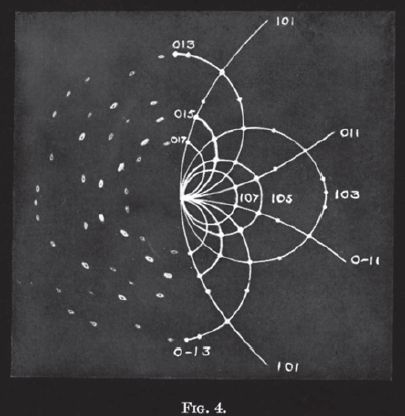
\includegraphics[width=0.4\linewidth]{Captură de ecran 2025-04-21 164501.png}
    \caption{Intersection of dots match ellipsis corresponding to the selected planes}
    \label{fig:elipses}
\end{figure}


Notice how for a reflection to be observed, the coordinates must be all odd or all even. Having $h_1, h_2, h_3$ the phase at a certain atom, WLB describes
$$\frac{\lambda}{2a}=\frac{2h_2}{\sqrt{h^2_1+h^2_2+h^2_3}}$$
and his observations regarding this formula explain the intensity and the possible presence or absence of a certain spot, even though he admits that other explanations may also be possible. In his notes, he states that $\frac{a}{\lambda}$ must be in a certain range defined by the values of \textit{h} and within this range, the intensity of the spot is the highest in the middle and faints towards the edges. In order to prove this, he analysed a crystal in symmetric form and when it is tiled 3°. For a point in the plane defined by the points $(0,0,0), (3a,0,a), (0,3a,a)$ the corresponding spot has a higher intensity in the tilled form $(\frac{\lambda}{a}=6.5)$ than in the symmetric form $(\frac{\lambda}{a}=4.3)$.\\
It is also explained how no other arrangement of molecules offer a complete series of points and it also fits with other models for the ZnS blades.

The same analysis can be performed for other crystal arrangements to confirm these observations. He asses a simpler crystal to show the elasticity of the X-Rays and the intensity dependence on $\lambda$, not only on the position of the plane.

In figure \ref{fig:exp} it is shown how the spots become more elliptical as the photographic plate is moved away from the crystal, proving that light is reflected and not channelled. This is probably the observation that made WLB realise the spots are formed by reflexion.
\begin{figure}[h]
    \centering
    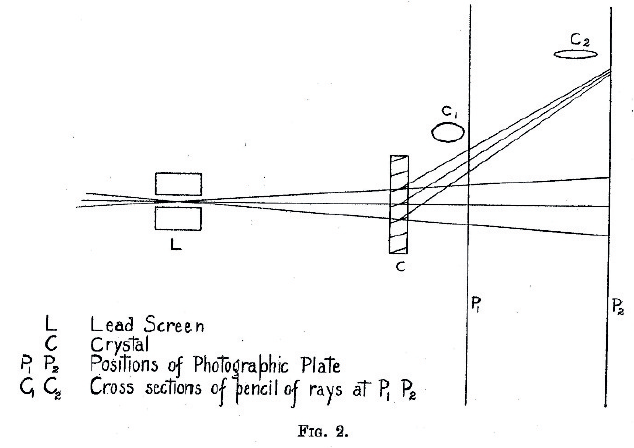
\includegraphics[width=0.5\linewidth]{Captură de ecran 2025-04-21 172516.png}
    \caption{Experiment set-up showing the reflexion of waves after passing through a crystal and the shape they get as they move further from the crystal}
    \label{fig:exp}
\end{figure}

Further experiments with crystals show which parameters of the crystals are relevant for the formation and characteristics of the spots.

\section{Bragg’s Law statement and proof}

\cite{Bragg} Bragg's Law states “when the X-ray is incident onto a crystal surface, its angle of incidence, $\Phi$, will reflect with the same angle of scattering, $\Phi$. And, when the path difference, \textit{d} is equal to a whole number, \textit{n}, of wavelength, $\lambda$, constructive interference will occur.”. The wavelengths that are re-emitted after hitting a plane interact with each other in a constructive or destructive way, forming a diffraction pattern on photographic plate. The wavelengths reflected are proportionate to the distance between the planes and depend on the angle of incidence after the formula $n\lambda=2d\sin{\Phi}$, where \textit{d} is the distance between planes, $\Phi$ the angle between the plane and the incident beam, and \textit{n} an integer (note how in his paper he used the angle between the normal and the incident beam, so his original formula is $\lambda=2d\cos{\theta}$).

Now, in order to prove this, multiple ways are possible. The geometric way refers to the dependence of the phase on the wavelength of the beam and calculates the necessary angle of incidence. Another way uses Laue’s equation and the condition for elastic interactions to derive Bragg’s Law.

In a crystal, atoms are arranged in a certain pattern, making its interaction with the X-ray predictable. Therefore, parts of the wave are spread in a different direction, while others pass in between. For the reflected waves to create a spot on the detector, they need to interfere constructively, which happens when they are in the same phase. We know from Laue's work\cite{Laue} that this happens when the path difference between different interacting atoms is an integer multiple of the wavelength. If the distance between 2 layers is \textit{d}, the extra distance travelled is $2d\sin{\Phi}$ . This distance must be equal to $n\lambda$ . And thus, the Bragg's Law.

Taking a more algebraic look at this, we need to consider $\vec{k}$ the wave vector, with the norm $\frac{2\pi}{\lambda}$, and $\lambda$ the wavelength of the particle. \gls{Laue's equation} says: 
$$\vec{k'}-\vec{k}=\vec{G}$$
Where $\vec{k'}$ is the reflected wavevector, $\vec{k}$ the incident vector, and $\vec{G}$ the reciprocal lattice vector. The difference vector needs to part of the crystal lattice for the interaction to be elastic (meaning that the 2 quotient spaces defined by the incident and reflected beam will be symmetric in rapport with the reflective plane). Connecting this to Bragg’s Law and using vector algebra 
\begin{gather*}
    \norm{\vec{G}}=\norm{\vec{k'}-\vec{k}}^2=\norm{\vec{k'}}+\norm{\vec{k}}-2\norm{\vec{k'}}\norm{\vec{k}}\cos{2\Phi} \\
    \norm{\vec{G}}^2=2\frac{4\pi^2}{\lambda^2}-2\frac{2\pi}{\lambda}\frac{2\pi}{\lambda}\cos{2\Phi}\\
    \norm{\vec{G}}=2\left(\frac{2\pi}{\lambda}\right)^2(1-\cos{2\phi})=4\left(\frac{2\pi}{\lambda}\right)^2\sin^2{\Phi}\\
    \norm{\vec{G}}=\frac{4\pi}{\lambda}\sin{\Phi}
\end{gather*}

but, according to imperical data\cite{lattice}
$$\norm{\vec{G}}=\frac{4\pi n}{d}$$
for a set of planes with distance d in between. Therefore:
$$n\lambda=2d\sin{Phi}$$
Using Schrödinger's Equation offers a broader understanding of the Law and the way it is used for non-crystalline structures in modern medical research. It shows how a particle behaves after interacting with a periodic structure such as a crystal and makes a connection between the unknown structure and the known diffraction pattern. The wavelike solution of the equation shows the condition that allows diffraction to happen in the first place.


\section{How to determine protein structure using X-Ray crystallography and Bragg's Law}

Using X-Ray crystallography for determining structures gives mostly straightforward solutions with high precision, being a useful tool for further mechanistic understanding. Although more complex than determining a crystal structure, proteins can also be solved with the same principles.
What we get from such an analysis is a diffraction pattern, as in figure \ref{fig:diff pattern}, and these patterns need to be interpreted. An electron density mas is determined using the Fourier transformation and finally, after many refinements made using plenty of statistical methods, the protein structure is determined.

\begin{figure}[h]
    \centering
    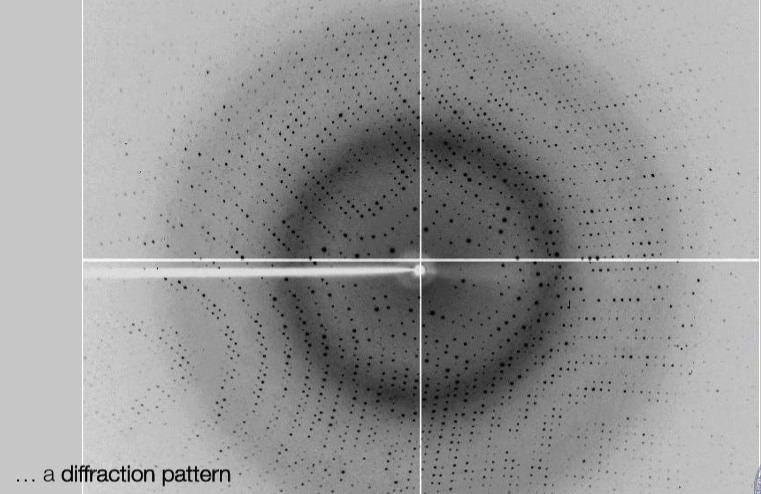
\includegraphics[width=0.5\linewidth]{Captură de ecran 2025-04-23 003653.png}
    \caption{Diffraction pattern obtained on a photographic plate after analysing a protein}
    \label{fig:diff pattern}
\end{figure}

The first step is to form a protein crystal, in order to make sure the structure is coherent and the x ray hits all the molecules from the same relative position. Next, Bragg’s Law is used to determine the interplanar spacing between crystal planes. The distance is reported to the \gls{Miller Indices} hkl, which are specific to certain crystal arrangements and help solve the equation: 
$$d_{hkl}=\frac{n\lambda}{2\sin{\phi}}$$
The reflection angle $\phi$ is calculated by a software that records the distance from the crystal to the detector \textit{L} and the position \textit{x} where the beam hits the detector. Then the angle can be calculated with the formula:
$$\phi=\frac{1}{2}\arctan{\frac{x}{L}}$$
Now, the electron density map can be modeled via Fourier transformation. The intensity of the diffraction spot is proportional to the square of the amplitude of the scattered wave, an observation that WLB also pointed out. With \textit{F(hkl)} being the structure factor, a complex number that represents the amplitude and the phase of the scattered X-Ray, $f_j$ the atomic factor (the probability of atom j to scatter X-Rays), and $(x_j, y_j, z_j)$ the coordinates of the atom j, the formula for the structure can be written like this:
$$F(hkl)=\sum_j f_je^{2\pi i(hx_j+ky_j+lz_j)}$$
The electron density inside the unit cel is of course, a real-space function, and the diffraction pattern gives a Fourier transformation in its reciprocal space. This tells us how much the structure scatters the wave in each direction. The electron cloud is converted into a set of wave components that describes diffraction intensities. Performing an inverse Fourier transformation computes the real space picture of the structure: 
$$F(hkl)=\int\int\int\rho(x,y,z)\cdot e^{-2\pi i(hx+ky+lz)}dxdydz$$
becomes $$\rho(x,y,z)=\frac{1}{V}\sum_{hkl}F(hkl)\cdot e^{2\pi i(hx+ky+lz)+i\phi_{hkl}}$$
And for the last step, the actual reconstruction of the electron density map is done by inserting the measured values of the intensities in the inverse Fourier transformation. The only problem with this method is that the phase of the beam is unknown and different models have to be tested. 

Even though, theoretically, the phase problem can be resolved, it does not come from experimental data and scientists can not be certain of its accuracy. The biggest techniques that solve this problem are molecular replacement, which uses the model of a protein with similar structure, multiple isomorphous replacement, where crystals with and without heavy atoms are grown and the differences in diffraction pattern help solve the phase problem mathematically, or anomalous dispersion, based on the propriety of some atoms to scatter X-Ray differently depending on the wavelength, and data at different wavelengths form a system for solving the phases. These are approximations, as data is always lost in huge analyses like this. In reality, the actual phase is more of a guessing game, and for this reason, statistics also play a major role in determining protein structures.

Therefore, even in a world where mathematics is assumably absent such as biology and biochemistry, we can see that the most fundamental concept would have been unknown to humankind without developments in mathematics such as solutions to Schrödinger's equation, Fourier transformation and statistics.

Bragg's Law, which seems to play a minor role in this concept, is in fact the starting point of what we know today about atomic structures, and nothing would have been possible without WLB and his father's observations regarding crystallography.

\printglossary[title=Notes]
\printbibliography[title={REFERENCES }, heading=bibintoc]

\end{document}